
A key property of our resource-rational lossy-context model is a close structural relationship between encodings $\representation$ and inputs $\contextInput$.
This is different from information-theoretic bottleneck models, which in general do not assume any structural correspondence between the input and the encoding \citep{tishby2000information}.

Here, we illustrate that a purely information-theoretic bottleneck does not predict the empirically observed bias towards surface-similar strings predicted by the resource-rational model.
We constructed a very simple and explicit probabilistic grammar that models some key aspects of the One and Two conditions, while being simple enough to permit exact calculations.
The grammar is shown in Figure~\ref{fig:grammar}; it generates sentences such as ``report annoyed patient'' and ``report that doctor annoyed patient startled janitor''.
Crucially, it incorporates a preference for ``report+PP'' over ``report+SC'', and ``fact+SC'' over ``fact+PP''.
We note that the grammar is extremely idealizing on purpose; it is intended not as a plausible model of human language, but to qualitatively showcase how certain properties of different models give rise to different predictions.


Using the method of Lagrange multipliers, our resource-rational objective function can be written 
\begin{equation}\label{eq:resource-toy}
\mathcal{L}_\textit{resource-rational}(\theta) = \operatorname{I}[\contextInput_{N+1}|\representation_{1\dots N}] + \kappa \cdot \mathbb{E}\left[\#\{i : \representation_i=\text{\textsc{erased}}\}\right]
\end{equation}
where the Lagrange multiplier $\kappa > 0$ depends on $\delta$, and maximizing $\mathcal{L}_\textit{resource-rational}(\theta)$ corresponds to solving (\ref{eq:objective-si}).

A corresponding information-theoretic bottleneck model is obtained by allowing arbitrary encodings $\representation$ (without a structural relationship with $\contextInput$), and constraining not the number of retained words, but the mutual information between inputs $\contextInput$ and encodings $\representation$.
The corresponding objective function thus reads:
\begin{align}\label{eq:bottleneck}
	\mathcal{L}_\textit{info-bottleneck}(\theta) & = \operatorname{I}[\contextInput_{N+1}|\representation] - \beta \cdot \operatorname{I}[\contextInput_{1\dots N} : \representation]
\end{align}
This objective function describes a \textbf{past-future} or \textbf{predictive information bottleneck} \citep{tishby2000information, Amir2015PastfutureIB, Marzen2016PredictiveRF, Still2010OptimalCI, Creutzig2009PastfutureIB, hahn2019estimating, Wang2019PastfutureIB}.
This describes the problem of compressing observed inputs $\contextInput_{1\dots N}$ into representations $\representation$ that maximize informativity about the future, while minimizing the number of encoded bits.
The parameter $\beta$ describes the strength of the pressure towards minimizing the number of encoded bits; it can take values $0 \leq \beta < 1$ ($\beta = 0$ corresponds to perfectly encoding $\contextInput$; $\beta\rightarrow 1$ corresponds to preserving no information about $\contextInput$ at all).

For each $\beta = 0.1, \dots, 0.9$, we solved~(\ref{eq:bottleneck}) for the grammar given in Figure~\ref{fig:grammar}, considering the setting where $\representation$ is a discrete random variable with up to 2,000 possible states.
For comparison, we also solved for the resource-rational model $Q$ (\ref{eq:objective-si}) using the same neural variational method as in our main simulation study; we represented the prior $P(\contextInput)$ using a trained LSTM instead of GPT-2.



We then calculated predicted surprisal of the final verb in all sentences of the form ``fact \textit{surprised}...'' and ``fact that doctor annoyed patient \textit{surprised}...''  that can be generated by varying nouns and verbs as given by the grammar.

We show the predicted surprisals in Figure~\ref{fig:bottleneck}.
The pattern of the resource-rational model agrees qualitatively with the results of the main simulations.
When encodings $\representation$ are most faithful, at low $\delta$ or $\beta$, both models shows a positive main effect of embedding bias in the One condition, and no effect in the Two condition. This agrees qualitatively with the conceptual predictions that we derived for Surprisal Theory.
In the resource-rational model, there is a range of $\delta$ where a negative main effect of embedding buas is observed in the Two condition -- this is a signature prediction of models exhibiting a bias towards surface-similar strings.
In the information bottleneck model, as $\beta$ increases ($\beta \geq 0.4$), the effect in the One condition disappears until, for very large $\beta$ ($\beta \geq 0.7)$, the difference between the One and Two condition also disappears.
Crucially, there provably is no range of $\beta$ where embedding bias shows a negative main effect in the Two condition in the Information Bottleneck model.

Fundamentally, the information-theoretic bottleneck method does not show a bias towards surface-similar strings because there is no constraint encouraging similar representations $\representation$ for surface-similar strings. For instance, under the information-theoretic bottleneck model, ``report that doctor annoyed patient'' is mapped to the same code $\representation$ as ``\textbf{fact} that doctor annoyed patient'', as these prefixes have exactly the same possible completions under the grammar.
In contrast, it is never mapped to the same $\representation$ as ``report \textbf{about} doctor annoyed patient'' unless $\beta$ is very close to $1$.

Yet another modeling option could maintain structured representations $\representation_{1\dots N}$ as in our model, but combine these with the information-bottleneck objective~(\ref{eq:bottleneck}).
Such a model would preferentially delete low-frequency and content words, as this would decrease $\operatorname{I}[\contextInput_{1\dots N} : \representation]$ the most.
We consider such a model implausible, as it would contravene well-established findings about word frequency effects in human memory \citep{Gorman1961RecognitionMF,Glanzer1976AnalysisOT}.

We note that, while the presence of a structural relationship between context and memory representations is particularly evident in our model, this is a property shared with previous psycholinguistic model of sentence comprehension.
For instance, in models of retrieval-based parsing \citep{lewis2005activation}, memory representations consist of chunks, each of which describes some part of the syntactic structure and originates when processing one of the words in the input. The layout of representations is thus tightly linked to the layout of the input, quite distinct from the structure-less compression created by an information bottleneck model.
Whereas this might be viewed as an incidental consequence of the use of an incremental parsing algorithm in models such as \citet{lewis2005activation}, our experimental results suggest that such a correspondence between representations and input may in fact be a key aspect of human syntactic processing.



\begin{figure}
    \centering
    \begin{tabular}{ccl}
    Resource-Rational  & Information Bottleneck \\
    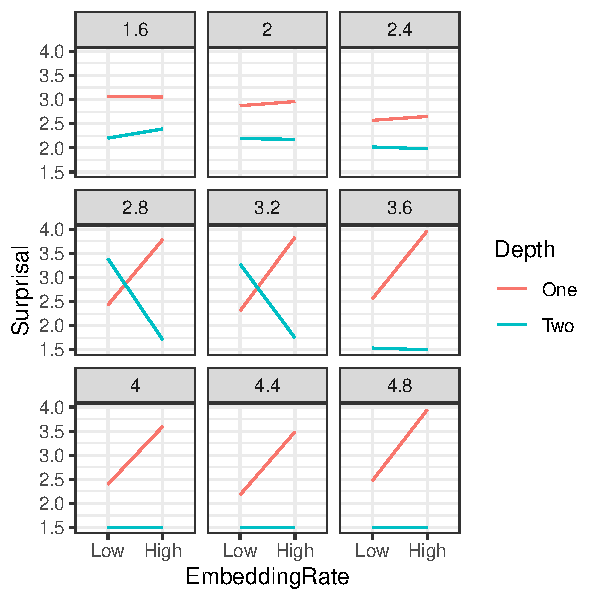
\includegraphics[width=0.4\textwidth]{figures/resource-rational_Integer.pdf} &
    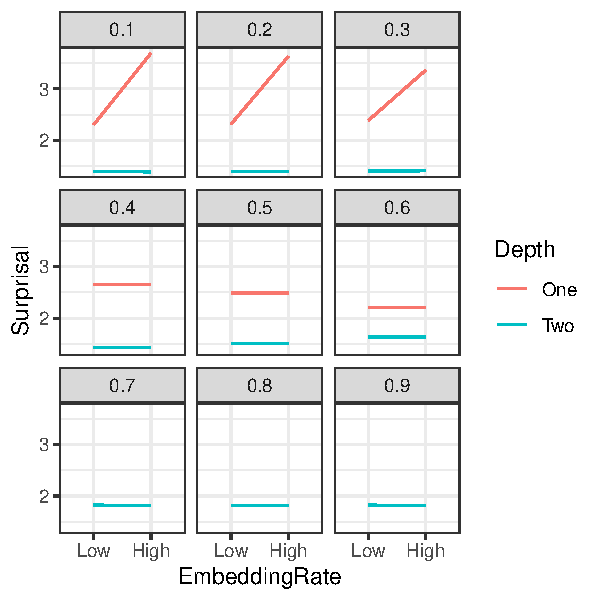
\includegraphics[width=0.4\textwidth]{figures/bottleneck.pdf}
    \end{tabular}
    \caption{Surprisals on the last verb in the miniature language (Figure~\ref{fig:grammar}) under the resource-rational surprisal model as a function of $\delta$ (left) and an information-theoretic bottleneck as a function of $\beta$ (right).}
    \label{fig:bottleneck}
\end{figure}


\begin{figure}
    \centering
    \begin{tabular}{|lll|l|l|lllll}
    \hline
  &              &          & $p$ & Examples \\ \hline\hline
S &$\rightarrow$ & NP$_1$ VP EOS & 0.5 &  fact annoyed  patient.\\
S &$\rightarrow$ & NP$_2$ VP EOS & 0.5 &  report annoyed  patient.\\
\hline
NP$_1$ & $\rightarrow$ & N$_1$ &  0.1 &  fact \\
NP$_1$ & $\rightarrow$ & N$_1$ SC &  0.7 &  fact that doctor annoyed  patient\\
NP$_1$ &$\rightarrow$ & N$_1$ PP &  0.2 &  fact about  doctor\\
\hline
NP$_2$ & $\rightarrow$ & N$_2$ &  0.4 &  report \\
NP$_2$ & $\rightarrow$ & N$_2$ SC &  0.1 &  report that doctor annoyed patient\\
NP$_2$ &$\rightarrow$ & N$_2$ PP &  0.5 &  report about doctor\\
\hline
NP$_3$ &$\rightarrow$ & N$_3$ & 0.25 & doctor\\
\hline
PP &$\rightarrow$ & about NP$_3$ & 1 & about doctor\\
\hline
SC &$\rightarrow$ & that NP$_3$ VP & 1 & that doctor annoyed patient\\
\hline
VP &$\rightarrow$ & V NP$_3$ & 1 & annoyed doctor\\
\hline
$N_1$ & $\rightarrow$ & fact, belief, $\dots$ & uniform & fact \\
$N_2$ & $\rightarrow$ & report, story, $\dots$ & uniform & report \\
$N_3$ & $\rightarrow$ & doctor, patient, $\dots$ & uniform & doctor \\
V & $\rightarrow$ & annoyed, shocked, surprised, pleased, $\dots$ & uniform & annoyed \\
\hline
    \end{tabular}
    \caption{Probabilistic grammar describing a fragment containing the \textsc{One} and \textsc{Two} conditions, restricted to the \textsc{Compatible} condition. For each of open word classes $N_1, N_2, N_3, V$, we assumed 10,000 distinct words.}
    \label{fig:grammar}
\end{figure}



